\section{BFS-array based implementation}
\label{sec:bfsimpl}

Based on the idea of partial tree, we can divide a large XML document into
chunks and distribute the evaluation of XPath queries over partial trees
constructed from the chunks of the document. However, without appropriate
implementation, it is still difficult to process XML document efficiently in
case when they are large. This is because the requirements for processing the
large XML documents are more strict, particularly that the memory and random
access to tree nodes become more crucial.

Indexing is a common used technique in database community for efficient aceess
of data~\cite{JLWO03,PCSS04}. Agarwal et al~\cite{AgKS15} proposed an idea for
processing queries on compresssed XML data for memory efficiency. While Krulis
et al~\cite{KrYa10} studied how to process queries on multi-core.  In this
section, we propose an effecient implementation of partial tree based on two
indexes: BFS-array index and grouped index in considering the characteristic of
partial tree. For better use, we also introduce attribute nodes and values of
nodes into our implementation.

To begin with, we give an example first. Considering the following XML document
that has been divided into four chunks as an example, an XML tree can be
constructed from the XML document as shown in Figure~\ref{fig:bfstree}.

\begin{flushleft}
	chunk$_0$:~\texttt{<r><b><d><c>txt1</c></d><a at="1"></a></b><b><d>}\\
	chunk$_1$:~\texttt{<c>txt2</c><d><c>txt3</c></d></d><a at="2"></a><d>}\\
	chunk$_2$:~\texttt{<c>txt4</c><c>txt5</c></d><a at="3"></a></b><b><d>}\\
	chunk$_3$:~\texttt{<c>txt6</c></d><d><d><c>txt7</c></d></d></b></r>}
\end{flushleft}

In this XML document, there are three attributes and seven text values. An
attributes is denoted as a rectangle boxes with both the attribute name and the
attribute value. The Value of a node is denoted as a rectangle box with only
the text of the node.

Now, let us consider how partial tree work for this XML document that has four
chunks. Since attribute nodes are inside a tag, which will not be separated, and
the values of nodes that can be considered as a regular tree node, there is no
difference in applying partial tree. We then can construct four partial trees as
shown in Figure~\ref{fig:bfspartialtree}.

\begin{figure}[t]
	\centering
	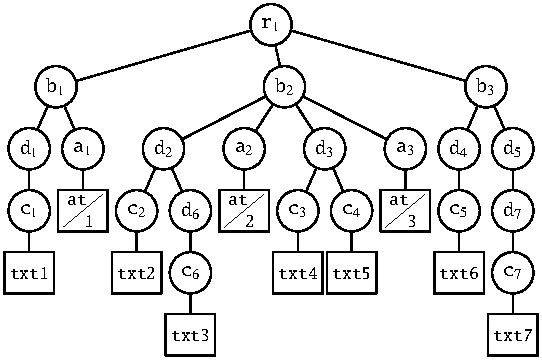
\includegraphics[scale=1.1]{partialtree/figures/bfstree.pdf}
	\caption{An example XML tree with values.}
    \label{fig:bfstree}
\end{figure}

\begin{figure}[t]
	\centering
	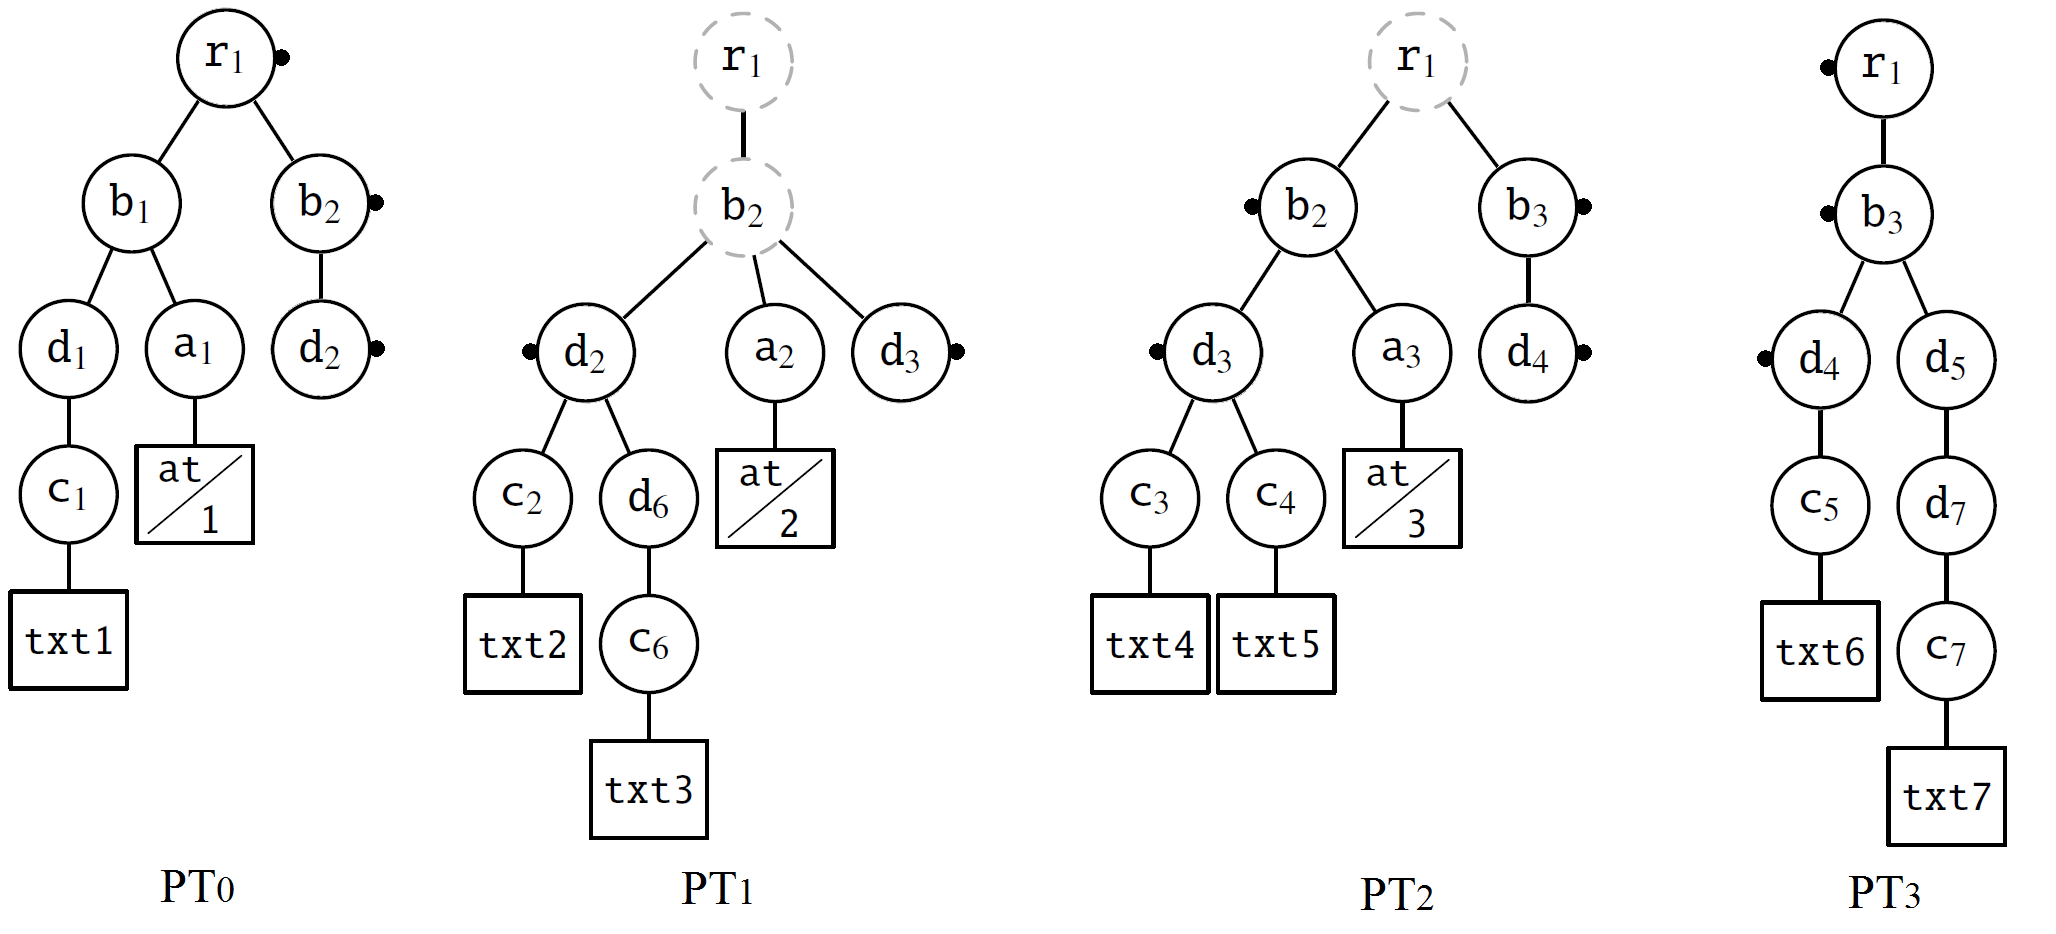
\includegraphics[scale=0.26]{partialtree/figures/bfstrees.png}
	\caption{Partial trees with values from the XML document.}
	\label{fig:bfspartialtree}
\end{figure}

For the four partial trees, we represent element nodes, attribute nodes and
value nodes consistent as the original XML tree. Since the partition only
affects the element node, from which the open nodes are only generated and
attribute nodes and content nodes can be simply implementated by the idea of
partial tree. As we have introduced in Section~\ref{sec:construction}, the split
tags are merged in case when the split position falls inside a tag and thus
splits the tag into two halves. In case of a text node is split into two sub
texts and separated on different partial trees, we simply merge the split two
sub texts into one and leave it on one partial tree. Thus this makes the
algorithm consistent.

The partial trees in the previous section provide a nice fragmentation of an XML
tree, making it possible for data parallel processing. To develop a
high-performance query framework, we still need to design concrete data
representation taking the following two issues into consideration.

\textbf{Expressiveness}

Originally indexing (or labeling) was considered to put shredded XML data into
databases~\cite{BGvM06,OOPC04}, but its expressiveness is very important to
accelerate queries.

\textbf{Compactness}

In the case we repeatedly apply several queries on the same data, we can put all
the indices in memory to avoid expensive I/O cost.

The first design choice is about the updates of XML data. In general purpose
framework, efficient support of updates is an important issues and several
frameworks support updates with sophisticated indexing such as
ORDPATH~\cite{OOPC04}. However, such an index with the update capability tends
to be large and complicated to handle. In this study, we decided not to allow
users to update XML data, which makes the implementation much simpler and
faster. We expect that users can fulfill their objective without updating the
XML data themselves,  if we provide some programming interface over the
framework.

The second design choice is about the functionality that the indices provide. An
important goal of this work is to support queries with not only the
\texttt{child} and \texttt{descendant} axes but also order-aware ones such as
\texttt{following-sibling} and \texttt{following}. To achieve our goal, the
following functions should be efficiently implemented.

\begin{figure*}[t]
	\centering
	\begin{minipage}{.2\linewidth}
		Partial tree\\[15pt]
		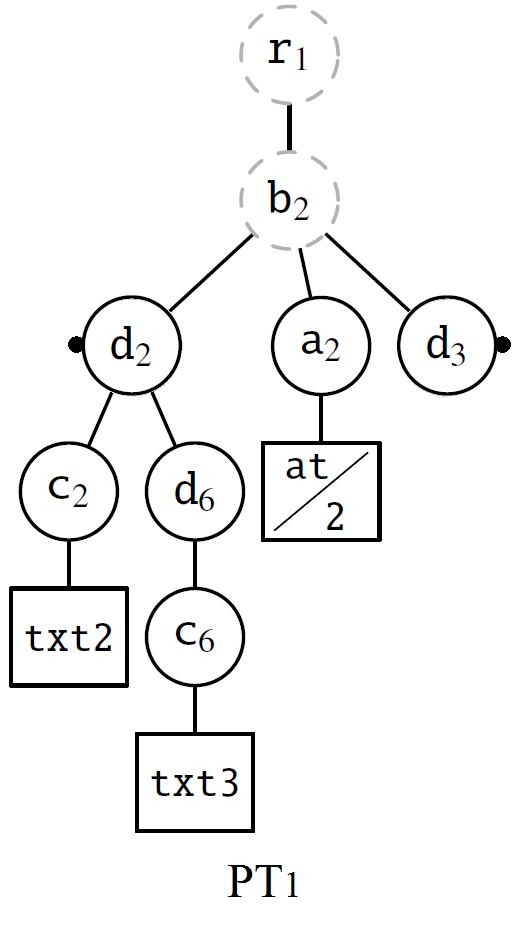
\includegraphics[scale=.25]{partialtree/figures/bfspt1.png}
	\end{minipage}
	\begin{minipage}{.55\linewidth}
		BFS-array \\
		\begin{tabular}{c|lcrrrr}
			\hline
			index   & tag             & type &  st & ed  & par    &  ch \\
			\hline
			1  & 5 (\texttt{r})  & N-OO &  0  & 196 &   0    &  2  \\
			2  & 2 (\texttt{b})  & N-OO & 42  & 142 &   1    &  3  \\
			3  & 4 (\texttt{d})  & N-OC & 45  &  81 &   2    &  6  \\
			4  & 1 (\texttt{a})  & N-CC & 81  &  95 &   2    &  8  \\
			5  & 4 (\texttt{d})  & N-CO & 95  & 124 &   2    &  9  \\
			6  & 3 (\texttt{c})  & N-CC & 48  &  59 &   3    &  9  \\
			7  & 4 (\texttt{d})  & N-CC & 59  &  77 &   3    & 10  \\
			8  & 6 (\texttt{at}) & A    & 88  &  88 &   4    & 11  \\
			9  & 0               & T    & 51  &  55 &   6    & 11  \\
			10 & 3 (\texttt{c})  & N-CC & 62  &  73 &   7    & 11  \\
			11 & 0               & T    & 65  &  69 &  10    & 12  \\
			\hline
		\end{tabular}
	\end{minipage}
    \begin{minipage} {.2\linewidth}
    Grouping Array \\[15pt]
 	\begin{tabular}{c|l}
 	\hline
 	tag  &   index      \\
 	\hline
 	0  &  $[9, 11]$ \\
 	1  &  $[4]$ \\
 	2  &  $[2]$ \\
 	3  &  $[6]$  \\
 	4  &  $[3,5,7]$  \\
 	5  &  $[1]$  \\
 	6  &  $[8]$  \\
 	\hline
    \end{tabular}
\end{minipage}
	\caption{A partial tree and its representation with two arrays}
	\label{fig:2arrays}
\end{figure*}

\begin{itemize}
	\item Function $\mathsf{getChildren}(x)$ returns all the children of node $x$.
	\item Function $\mathsf{getParent}(x)$ returns the parent of node $x$.
	\item Function $\mathsf{nextSibling}(x)$ returns the next (right) sibling of node $x$.
	\item Function $\mathsf{prevSibling}(x)$ returns the previous (left) sibling of node $x$.
	\item Function $\mathsf{isDescendant}(x, y)$ returns true if node $x$ is a descendant of node $y$.
	\item Function $\mathsf{isFollowing}(x, y)$ returns true if node $x$ is strictly after node $y$ in the document order.
	\item Function $\mathsf{getNodesIn}(t, x)$ returns all the nodes with tag $\mathit{t}$ in the subtree rooted at $x$.
\end{itemize}

We design two index sets (Fig.~\ref{fig:2arrays}) to provide these functions
keeping the indices compact. A node has the following fields:

\begin{itemize}
	\item $\mathit{tag}$: tag names (they are short integers that map to the strings),
	\item $\mathit{type}$: type of nodes including the four node types,
	\item $\mathit{st}$: start position (the position in the file to avoid global counting), and
	\item $\mathit{ed}$: end position.
\end{itemize}

The first index, \emph{BFS-array}, lists all the nodes in the order of the
breadth first search (BFS). Every node has two integer pointers to its parent
($par$) and the first child ($ch$) in this list. With the BFS order and these
two pointers, we can compute functions $\mathsf{getChildren}$,
$\mathsf{getParent}$, $\mathsf{nextSibling}$, and $\mathsf{prevSibling}$
efficiently. The second index, \emph{Grouped-array}, groups the nodes by their
tag names and then sorts the nodes in the groups by their start position.  With
this index, we can evaluate the function $\mathsf{getNodesIn}$ efficiently.

In our implementation, we used
2 bytes for $\mathit{tag}$,
1 bytes for $\mathit{type}$,
8 bytes for $\mathit{st}$,
8 bytes for $\mathit{ed}$,
4 bytes for $\mathit{par}$,
4 bytes for $\mathit{ch}$, and
4 bytes for $\mathit{idx}$.
(Though total file size could exceeds 32 bits, we assume that the number of
elements in a single partial tree can fit in 32 bits.) The total size needed for
representing a node is $2 + 1 + 8 + 8 + 4 + 4 + 4 = 31$ bytes, which is much
smaller than several implementation of DOM trees or databases. This is a key to
achieve high-performance evaluation of queries.
